
\documentclass{article}
\usepackage{hyperref}
\usepackage{verbatim}
\usepackage{graphicx}
\usepackage{xcolor}
\usepackage{tikz}
\usepackage{lscape}
\usepackage{pgfgantt}
\usepackage{cleveref}
\usepackage[a4paper,margin=1in]{geometry}
\usetikzlibrary{patterns}
\usetikzlibrary{calc}
\usetikzlibrary{decorations.pathmorphing}
\usetikzlibrary{shapes}
% \usepackage{url}
\usepackage{wrapfig}
\usepackage[numbers]{natbib}
\newcommand{\itm}[1]{\begin{itemize} #1 \end{itemize}}
\newcommand{\num}[1]{\begin{enumerate} #1 \end{enumerate}}
\newcommand{\sctn}[1]{\section{#1} }
\newcommand{\ssctn}[1]{\subsection{#1} }
\newcommand{\sssctn}[1]{\subsubsection{#1} }
\newcommand{\img}[2]{\includegraphics[scale=#1]{#2}}
\newcommand{\rarr}{$\rightarrow$ }
\newcommand{\bld}[1]{\textbf{#1}}
\newcommand{\itl}[1]{\textit{#1}}
\newcommand{\ctr}[1]{\begin{center} #1 \end{center}}
\newcommand{\fig}[3]{\ctr{\begin{figure}[htbp] #1 \caption{#2} \label{fig: #3} \end{figure}}}
\newcommand{\wrp}[1]{\begin{wrapfigure}{r}{0.25\textwidth}
						\centering
							#1
					 \end{wrapfigure}}

\newcommand\ytl[2]{
\parbox[b]{8em}{\hfill{\color{black}\bfseries\sffamily #1}~$\cdots\cdots$~}\makebox[0pt][c]
{$\bullet$}\vrule\quad \parbox[c]{12.5cm}
{\vspace{8pt}\color{black!40!black!80}\raggedright\sffamily #2.\\[15pt]}\\[-3pt]}

\title{KoMoDo++ Questionnaire}
\author{Applicant \_\_\_\_\_\_\_\_\_\_}
\date{}
%
%
%
\begin{document}
\pagenumbering{gobble}
\maketitle{}
\sctn{Instructions}
Please read questions carefully. Questions which have a range of answers only require one circle to be selected. 1 is considered the worst / slowest /hardest and 10 is considered the best / fastest / easiest.
\sctn{Tasks}
	\ssctn{Task 1}
	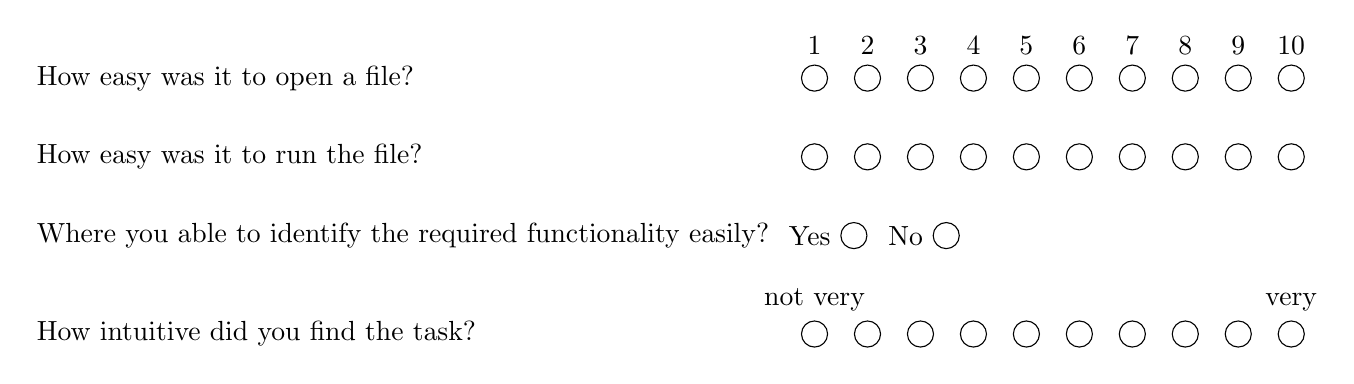
\begin{tikzpicture}[>=latex]
		%Question 1
		\node [right] at (0,0) (q1)[] {How easy was it to open a file?};
		\node at (canvas cs:x= 10cm,y=0cm)   (t) [circle,draw=black!100, minimum width=2mm] {};
		\node [above] at (t.north) {1};
		\foreach \x in {2,3,...,10}{
			% \pgfmathparse{\x - 5};
			\node at ($(t.east) + (0.5cm, 0cm)$)   (t) [circle,draw=black!100, minimum width=2mm] {};
			\node [above] at (t.north) {\x};
		}

		% Question 2
		\node[right] at (0,-1) (q2)[] {How easy was it to run the file?};
		\node at (canvas cs:x= 10cm,y=-1cm)   (t) [circle,draw=black!100, minimum width=2mm] {};
		% \node [above] at (t.north) {1};
		\foreach \x in {2,3,...,10}{
			% \pgfmathparse{\x - 5};
			\node at ($(t.east) + (0.5cm, 0cm)$)   (t) [circle,draw=black!100, minimum width=2mm] {};
			% \node [above] at (t.north) {\x};
		}

		% Question 4
		\node[right] at (0,-2) (q2)[] {Where you able to identify the required functionality easily?};
		\node at (canvas cs:x= 10.5cm,y=-2cm)   (t) [circle,draw=black!100, minimum width=2mm] {};
		\node [left] at (t.west) {Yes};
		\node at ($(t.east) + (1cm, 0cm)$)   (t) [circle,draw=black!100, minimum width=2mm] {};
		\node [left] at (t.west) {No};

		% Question 5
		\node[right] at (0,-3.25) (q2)[] {How intuitive did you find the task?};
		\node at (canvas cs:x= 10cm,y=-3.25cm)   (t) [circle,draw=black!100, minimum width=2mm] {};
		\node [above] at (t.north) {not very};
		\foreach \x in {2,3,...,9}{
			% \pgfmathparse{\x - 5};
			\node at ($(t.east) + (0.5cm, 0cm)$)   (t) [circle,draw=black!100, minimum width=2mm] {};
			% \node [above] at (t.north) {\x};
		}
		\node at ($(t.east) + (0.5cm, 0cm)$)   (t) [circle,draw=black!100, minimum width=2mm] {};
		\node [above] at (t.north) {very};

	\end{tikzpicture}
\ssctn{Task 2}
	
\begin{tikzpicture}[>=latex]
		%Question 1
		\node[right] at (0,0) (q2)[] {How did you find the level of feedback given at each step?};
		\node at (canvas cs:x= 10cm,y=0cm)   (t) [circle,draw=black!100, minimum width=2mm] {};
		\node [above] at (t.north) {unclear};
		\foreach \x in {2,3,...,9}{
			% \pgfmathparse{\x - 5};
			\node at ($(t.east) + (0.5cm, 0cm)$)   (t) [circle,draw=black!100, minimum width=2mm] {};
			% \node [above] at (t.north) {\x};
		}
		\node at ($(t.east) + (0.5cm, 0cm)$)   (t) [circle,draw=black!100, minimum width=2mm] {};
		\node [above] at (t.north) {clear};


		% Question 2
		\node[right] at (0,-1) (q2)[] {How clear were the changes in each step?};
		\node at (canvas cs:x= 10cm,y=-1cm)   (t) [circle,draw=black!100, minimum width=2mm] {};
		\node [above] at (t.north) {unclear};
		\foreach \x in {2,3,...,9}{
			% \pgfmathparse{\x - 5};
			\node at ($(t.east) + (0.5cm, 0cm)$)   (t) [circle,draw=black!100, minimum width=2mm] {};
			% \node [above] at (t.north) {\x};
		}
		\node at ($(t.east) + (0.5cm, 0cm)$)   (t) [circle,draw=black!100, minimum width=2mm] {};
		\node [above] at (t.north) {clear};
	\end{tikzpicture}
\ssctn{Task 3}
	
\begin{tikzpicture}[>=latex]
		%Question 1
		\node [right,text width=7.5cm]at (0,0) (q1)[] {Where you able to identify the reason for the error?};
		\node at (canvas cs:x= 10.5cm,y=0cm)   (t) [circle,draw=black!100, minimum width=2mm] {};
		\node [left] at (t.west) {Yes};
		\node at ($(t.east) + (1cm, 0cm)$)   (t) [circle,draw=black!100, minimum width=2mm] {};
		\node [left] at (t.west) {No};


		% Question 2
		\node[right] at (0,-1.25) (q2)[] {How helpful where the messages?};
		\node at (canvas cs:x= 10cm,y=-1.25cm)   (t) [circle,draw=black!100, minimum width=2mm] {};
		\node [above] at (t.north) {not very};
		\foreach \x in {2,3,...,9}{
			% \pgfmathparse{\x - 5};
			\node at ($(t.east) + (0.5cm, 0cm)$)   (t) [circle,draw=black!100, minimum width=2mm] {};
			% \node [above] at (t.north) {\x};
		}
		\node at ($(t.east) + (0.5cm, 0cm)$)   (t) [circle,draw=black!100, minimum width=2mm] {};
		\node [above] at (t.north) {very};

		% Question 3
		\node[right] at (0,-2) (q2)[] {Did you find it easy to use breakpoints?};
		\node at (canvas cs:x= 10.5cm,y=-2cm)   (t) [circle,draw=black!100, minimum width=2mm] {};
		\node [left] at (t.west) {Yes};
		\node at ($(t.east) + (1cm, 0cm)$)   (t) [circle,draw=black!100, minimum width=2mm] {};
		\node [left] at (t.west) {No};
	\end{tikzpicture}
\ssctn{Additional comments}
	\_\_\_\_\_\_\_\_\_\_\_\_\_\_\_\_\_\_\_\_\_\_\_\_\_\_\_\_\_\_\_\_\_\_\_\_\_\_\_\_\_\_\_\_\_\_\_\_\_\_\_\_\_\_\_\_\_\_\_\_\_\_\_\_\_\_\_\_\_\_\_\_\_\_\_\_\_\_\_\_\_\_\_\_\_\_\_\_\_\_\_\_\_\_\_\_\_\_\_\_\_\_\_\_\_\_\_\_\_\_\_\_\_\_\_\_\_\_\_\_\_\_\_\_\_\_
	\\\_\_\_\_\_\_\_\_\_\_\_\_\_\_\_\_\_\_\_\_\_\_\_\_\_\_\_\_\_\_\_\_\_\_\_\_\_\_\_\_\_\_\_\_\_\_\_\_\_\_\_\_\_\_\_\_\_\_\_\_\_\_\_\_\_\_\_\_\_\_\_\_\_\_\_\_\_\_\_\_\_\_\_\_\_\_\_\_\_\_\_\_\_\_\_\_\_\_\_\_\_\_\_\_\_\_\_\_\_\_\_\_\_\_\_\_\_\_\_\_\_\_\_\_\_\_
	\\\_\_\_\_\_\_\_\_\_\_\_\_\_\_\_\_\_\_\_\_\_\_\_\_\_\_\_\_\_\_\_\_\_\_\_\_\_\_\_\_\_\_\_\_\_\_\_\_\_\_\_\_\_\_\_\_\_\_\_\_\_\_\_\_\_\_\_\_\_\_\_\_\_\_\_\_\_\_\_\_\_\_\_\_\_\_\_\_\_\_\_\_\_\_\_\_\_\_\_\_\_\_\_\_\_\_\_\_\_\_\_\_\_\_\_\_\_\_\_\_\_\_\_\_\_\_
	\\\_\_\_\_\_\_\_\_\_\_\_\_\_\_\_\_\_\_\_\_\_\_\_\_\_\_\_\_\_\_\_\_\_\_\_\_\_\_\_\_\_\_\_\_\_\_\_\_\_\_\_\_\_\_\_\_\_\_\_\_\_\_\_\_\_\_\_\_\_\_\_\_\_\_\_\_\_\_\_\_\_\_\_\_\_\_\_\_\_\_\_\_\_\_\_\_\_\_\_\_\_\_\_\_\_\_\_\_\_\_\_\_\_\_\_\_\_\_\_\_\_\_\_\_\_\_
	\\\_\_\_\_\_\_\_\_\_\_\_\_\_\_\_\_\_\_\_\_\_\_\_\_\_\_\_\_\_\_\_\_\_\_\_\_\_\_\_\_\_\_\_\_\_\_\_\_\_\_\_\_\_\_\_\_\_\_\_\_\_\_\_\_\_\_\_\_\_\_\_\_\_\_\_\_\_\_\_\_\_\_\_\_\_\_\_\_\_\_\_\_\_\_\_\_\_\_\_\_\_\_\_\_\_\_\_\_\_\_\_\_\_\_\_\_\_\_\_\_\_\_\_\_\_\_
\end{document}
